\documentclass{../local}

\title{\textbf{Active Emergency Evacuation using Wireless Sensor Networks}}
\author{\\
		Hogeschool Utrecht\\
		\\
		Roy Scheefhals - 1563303}

\begin{document}

\begin{titlepage}
\begin{center}

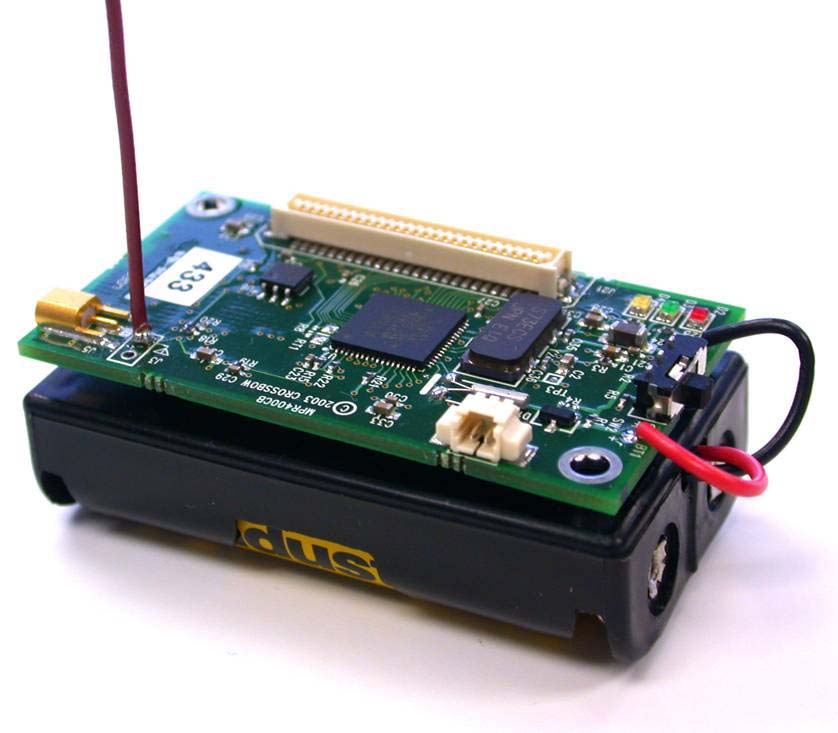
\includegraphics[width=0.6\textwidth]{mica2}~\\[1cm]

{ \huge \bfseries Active Emergency Evacuation using Wireless Sensor Networks \\[0.4cm] }
\hrule
\hspace{0pt} \\[1.3cm]

\begin{minipage}{0.4\textwidth}
\begin{flushleft} \large
\emph{Author:}\\
Roy \textsc{Scheefhals}\\
\emph{Hogeschool Utrecht}
\end{flushleft}
\end{minipage}
\begin{minipage}{0.4\textwidth}
\begin{flushright} \large
\emph{Bedrijfsbegeleider:} \\
Martin \textsc{Klomp}\\
\emph{Alten PTS}
\end{flushright}
\end{minipage}

\end{center}
\end{titlepage}

\newpage

\renewcommand{\thesection}{\Roman{section}}

\section*{Versiebeheer}
\begin{tabular}{ | l | l | l | p{7.5cm} |}
\hline
Versie & Wanneer & Wat \\ \hline
0.1 & 05-03-2014 & Eerste opzet document\\ \hline
0.2 & 07-03-2014 & Achtergrond Project v1\\ \hline
1.0 & 31-03-2014 & Eerste versie\\ \hline

\end{tabular}

\chapter{Inleiding}
\subfile{Inleiding}
\newpage\null\thispagestyle{empty}

\renewcommand{\thesection}{\arabic{section}}

% inhoud
\renewcommand*\contentsname{Inhoud}
\thispagestyle{empty}
\setcounter{page}{0}
\tableofcontents
\clearpage

\chapter{Achtergrond van Project} 
\subfile{Achtergrond}

\chapter{Opdracht Definitie}
\subfile{Opdracht}

\chapter{Planning en Aanpak}
\subfile{Planning-aanpak}

%References
%\bibliographystyle{plain}
%\bibliography{bib}
\subfile{Bibliography}

%\begin{appendices}
%\subfile{Appendix}
%\end{appendices}

\end{document}
